Super-resolution (SR) is a collection of methods\anote{vbsuper} that augment the resolving power of an imaging system.
%
Here, and in the forthcoming, by resolving power we mean the ability of an imaging device to distinguish distinct but proximal objects in a scene.
%
If such objects are modeled as point sources of light then the resolving power of the imaging system is defined by Rayleigh's criterion: two point sources are considered \textit{resolved} when the first diffraction maximum\anote{rayleighscriterion} of one point source (at most) coincides with the first minimum of the other (see figure~\ref{fig:rayleigh}).
\begin{figure}
	\center
	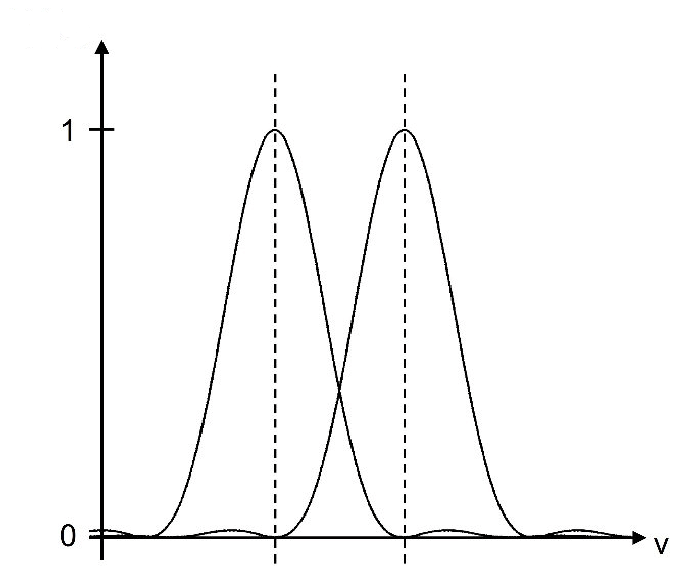
\includegraphics[width=\linewidth,keepaspectratio]{figures/classical/rayleigh.png}
	\caption{Rayleigh's criterion\cite{rayleigh}.}
	\label{fig:rayleigh}
\end{figure}

SR techniques yield high-resolution (HR) images from one or more observed low-resolution (LR) images by restoring lost fine details and reversing degradations produced by imperfect imaging systems.
%
In the case where a single LR source image is used to construct the HR correspondent, the techniques are referred to as single-image-super-resolution (SISR) techniques.
%
These techniques typically operate by either learning some mapping from low resolution chips (uniform partitions of the image, e.g. \(3\times 3\) pixels) to higher resolution chips that are highly similar (according to some metrics) and obey regularity constraints (e.g. agreement at edges).
%
In the case when multiple LR source images are used to construct the single HR correspondent, the techniques are referred to as multiple-image-super-resolution (MISR) techniques.
%
MISR techniques rely on non-redundant and yet pertinent information in multiple images of the same scene (see figure~\ref{fig:misr}).
\begin{figure}
	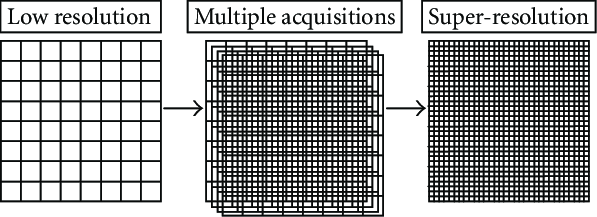
\includegraphics[width=\linewidth,keepaspectratio]{figures/classical/misr.png}
	\caption{Multiple image super resolution\cite{misr}.}
	\label{fig:misr}
\end{figure}
%
Note that for such information to exist there should be sub-pixel\anote{subpixel} shifts in either the imaging system or the scene between consecutive images.


For typical imaging use-cases, high resolution images are preferable to low resolution images; higher resolutions are
desirable in and of themselves and as inputs to later image processing transformations that can degrade image quality (e.g.\ by virtue of quantization or compression).
%
In theory the resolving power of an imaging system is primarily determined by the number of independent sensor elements that comprise that imaging system (each of which collects a component of the ultimate image).
%
Naturally then, a way to increase the resolution of such a system is to increase the density of such sensor elements per unit area.
%
Unfortunately, and counter-intuitively, since the number of photons incident on each sensor decreases as the sensor shrinks, shot noise\anote{shotnoise} thwarts that idea.
%
Furthermore, while sensor density is primary, secondary effects due to optics limit resolution as well;
the point spread of a lens (distortion of a point source due to diffraction), chromatic aberrations (distortion due to differing indices of refraction for differing wavelengths of light), and motion blur all function to obscure or erase details from the image.

In domains such as satellite/aerial photography, medical imaging, and facial recognition,
high-resolution reconstruction of low-resolution samples is eminently useful since ab-initio acquisition of high-resolution images is either logistically difficult or impossible due to aforementioned imaging apparatus limitations.
%
For example in the instance of satellite imagery, acquisition of high-resolution imagery is primarily hampered by optics and physics\anote{satelliteoptics}.
%
In contrast, in the cases of medical imaging (where procedures are invasive and patient exposure time needs to be minimized\cite{doi:10.1002.cmr.a.21249}) and facial recognition (e.g.\ for purposes of surveillance) the primary challenge is logistics and access to repeat collection opportunities.

The benefits of enhancing images using SR techniques include not only more pleasing or more readily interpretable images for human consumption but higher quality inputs for automated learning systems as well.
%
In particular object detection systems trained on super-resolved images outperform those trained on the low
resolution originals\cite{effectssuperres}.
%
Indeed this is our ultimate goal --- not super-resolution per se but super-resolution in the service of improved object detection performance for longwave-infrared (LWIR) imagery.
%
Note that while practically speaking, there exist hardware solutions for increasing the resolution of an imaging
system, we discount the value of such propositions.
%
We instead take low resolution images as given and seek techniques that allow for ex post facto reconstruction or inference of precise details.
%
This necessarily constrains techniques under consideration to be algorithmic in nature and software in practice.

The rest of this survey is outlined as follows: Section~\ref{sec:background} introduces imaging systems, notation, and the model of imaging that will be the mathematical framework for the proceeding sections, Section~\ref{sec:image-registration} surveys image registration techniques (a necessary pre-processing step for MISR), Section~\ref{sec:classical-algorithms} surveys classical techniques (those that do not employ neural networks), Section~\ref{sec:deep-learning-algorithms} surveys neural-network techniques with heavy emphasis on deep learning (i.e., deep networks), Section~\ref{sec:future-research} discusses the scope and goals of the author's research program, and Section~\ref{sec:conclusion} summarizes.
